\chapter{Benchmark Construction and Evaluation Protocol}

\section{Benchmark Construction}

Figure~\ref{fig:pipeline} summarizes the full protocol: two source tasks feed a rule-based romanizer, targeted human review freezes the validation-200 v5 core, a separately sampled and fully human-reviewed 974-row BEnQA extension provides scale, and both slices are evaluated with the same paired triad protocol.

\begin{figure}[H]
\centering
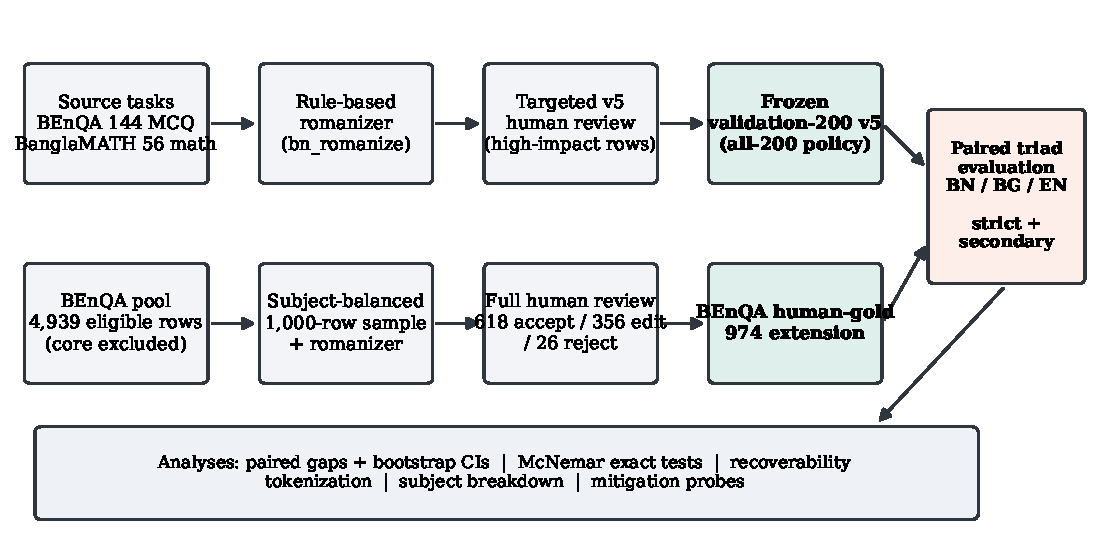
\includegraphics[width=\textwidth]{figures/fig_pipeline.pdf}
\caption{Benchmark construction and evaluation pipeline. The frozen validation-200 v5 core (top track) and the BEnQA human-gold 974 extension (bottom track) are evaluated under the same paired Bangla/Banglish/English protocol and shared analyses.}
\label{fig:pipeline}
\end{figure}

\subsection{Source tasks}

The benchmark construction has one goal: make script the main variable, not the question. To do this, the validation set combines two source tasks whose items can be represented in multiple script views while preserving the answer.

\textbf{BEnQA.} BEnQA contributes multiple-choice science questions. These items are well suited to paired script evaluation because the answer is a choice label and the same item can be represented in Bangla, Banglish, and English.

\textbf{BanglaMATH.} BanglaMATH contributes short-answer math word problems. These items stress numerical reasoning and answer normalization. They are harder to score strictly because correct answers may appear with units, Bengali digits, or intermediate reasoning.

The frozen validation-200 v5 slice contains 144 BEnQA items and 56 BanglaMATH items. The BEnQA subset is the cleanest source of script-gap evidence because choice-label scoring is less sensitive to answer formatting. BanglaMATH is kept as a stress-test slice because it exposes answer-compliance and numeric-unit issues that are important for deployment.

\subsection{Script variants}

Each item is represented in three main variants:

\begin{itemize}
\item \textbf{Bangla:} native Bengali script.
\item \textbf{Reviewed Banglish:} Latin-script Banglish after the v5 review pass.
\item \textbf{English:} English translation or English source variant.
\end{itemize}

All variants preserve the item id and gold answer. The prompt asks the model to return only the answer. For BEnQA, the expected output is one of A, B, C, or D. For BanglaMATH, the parser accepts short numeric or textual answers under strict and secondary modes. In other words, a script gap means the same item changes correctness when written differently; it does not mean that different questions were compared.

The English variant is useful but not identical in status to the Bangla-Banglish pair. English is a privileged comparison view. It helps identify whether an item is semantically answerable for a model, but the main orthographic claim is the Bangla-vs-reviewed-Banglish contrast.

\subsection{Review and denominator policy}

The v5 review pass targeted Banglish rows most likely to affect the thesis claim. After review, validation-200 v5 is frozen under an all-200 denominator policy. Three source-quality rows are also tracked under a strict-197 sensitivity view. The all-200 denominator remains primary because it avoids changing the evaluation set after seeing outcomes. The strict-197 view is a robustness check, not a replacement for the main result.

Review changed the main Banglish scores only slightly:

\begin{table}[H]
\centering
\caption{Review sensitivity from v4 Banglish to reviewed-v5 Banglish.}
\label{tab:review-sensitivity}
\small
\begin{tabular}{llll}
\hline
Model & v4 Banglish & reviewed-v5 Banglish & Change \\
\hline
Qwen2.5-3B & 39/200 & 41/200 & +1.0 pts \\
Qwen2.5-7B 8-bit & 48/200 & 47/200 & -0.5 pts \\
Qwen3-4B & 47/200 & 49/200 & +1.0 pts \\
\hline
\end{tabular}%
\end{table}

This is important. The review improves dataset quality but does not erase the script-conditioned weakness.

\section{Evaluation Protocol}

\subsection{Models}

The main open-model evaluation uses three compact Qwen instruction models:

\begin{itemize}
\item Qwen2.5-3B-Instruct
\item Qwen2.5-7B-Instruct in 8-bit
\item Qwen3-4B-Instruct
\end{itemize}

These models are small enough to run reproducibly on the available compute but strong enough to avoid a trivial ``all models fail everything'' result. They are therefore useful as thesis-facing baselines: failures are interpretable, but the experiments remain repeatable.

The frontier/API panel adds five hosted models:

\begin{itemize}
\item Gemini 3.5 Flash
\item GPT-5.5 low
\item Claude Sonnet 4.6
\item DeepSeek V4 Flash, non-thinking mode
\item Groq-hosted Llama 3.3 70B
\end{itemize}

The API rows use the same frozen validation-200 v5 prompt manifest and the same parser. They are not treated as a leaderboard. Their role is to test whether the Banglish gap disappears under stronger or differently trained systems.

\subsection{Scoring}

We report strict accuracy for all rows. Strict scoring measures whether the model produced the expected answer in a deployable form. For API rows we also report secondary parser/unit sensitivity. Secondary scoring gives credit for recoverable noncanonical answers, such as numeric-only answers with units or choice answers embedded in light markdown.

This separation is deliberate. Strict accuracy answers one deployment question: can the model follow the benchmark contract? Secondary accuracy answers a diagnostic question: did the model appear to know the semantic answer even if it violated the exact format?

\subsection{Paired gaps}

For each model and item, we compare correctness across script variants. The main gap is:

\texttt{reviewed Banglish accuracy - Bangla accuracy}

We also report:

\texttt{reviewed Banglish accuracy - English accuracy}

For the core Qwen rows and the human-reviewed BEnQA extension, we use paired bootstrap intervals. For the API validation panel, we also report exact paired sign-test style discordance summaries where available. Positive values mean Banglish is more accurate than the comparator. Negative values mean Banglish is less accurate.

\endinput
